\documentclass{extbook}[14pt]
\usepackage{multicol, enumerate, enumitem, hyperref, color, soul, setspace, parskip, fancyhdr, amssymb, amsthm, amsmath, bbm, latexsym, units, mathtools}
\everymath{\displaystyle}
\usepackage[headsep=0.5cm,headheight=0cm, left=1 in,right= 1 in,top= 1 in,bottom= 1 in]{geometry}
\pagestyle{fancy}
\lhead{}
\chead{Answer Key for Module\,7\,-\,Rational\,Functions Version B}
\rhead{}
\lfoot{Summer\,C\,2020}
\cfoot{}
\rfoot{}
\begin{document}
\textbf{This key should allow you to understand why you choose the option you did (beyond just getting a question right or wrong). \href{https://xronos.clas.ufl.edu/mac1105spring2020/courseDescriptionAndMisc/Exams/LearningFromResults}{More instructions on how to use this key can be found here}.}

\textbf{If you have a suggestion to make the keys better, \href{https://forms.gle/CZkbZmPbC9XALEE88}{please fill out the short survey here}.}

\textit{Note: This key is auto-generated and may contain issues and/or errors. The keys are reviewed after each exam to ensure grading is done accurately. If there are issues (like duplicate options), they are noted in the offline gradebook. The keys are a work-in-progress to give students as many resources to improve as possible.}

\rule{\textwidth}{0.4pt}

1. Choose the equation of the function graphed below.
\begin{center} 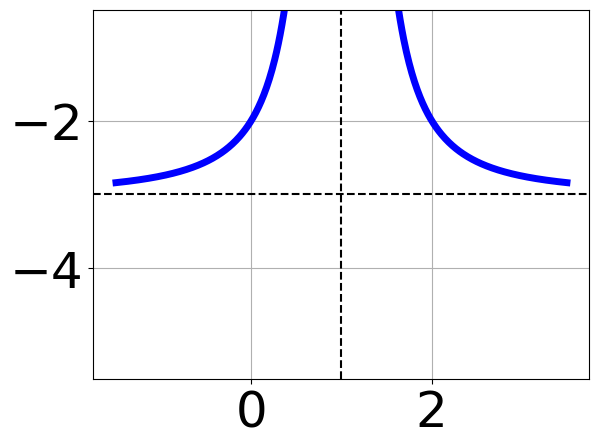
\includegraphics[width=0.3\textwidth]{../Figures/rationalGraphToEquationB.png} \end{center} 

The solution is $ f(x) = \frac{1}{x + 1} + 2 $ 

\begin{enumerate}[label=\Alph*.] 
\item $ f(x) = \frac{-1}{x - 1} + 2 $ 

 Corresponds to using the general form $f(x) = \frac{a}{x+h}+k$ and the opposite leading coefficient. 
\item $ f(x) = \frac{1}{(x + 1)^2} + 2 $ 

 Corresponds to thinking the graph was a shifted version of $\frac{1}{x^2}$. 
\item $ f(x) = \frac{1}{x + 1} + 2 $ 

 This is the correct option. 
\item $ f(x) = \frac{-1}{(x - 1)^2} + 2 $ 

 Corresponds to thinking the graph was a shifted version of $\frac{1}{x^2}$, using the general form $f(x) = \frac{a}{x+h}+k$, and the opposite leading coefficient. 
\item $ \text{None of the above} $ 

 This corresponds to believing the vertex of the graph was not correct. 
\end{enumerate} 
 
\textbf{General Comment:} General Comments: Remember that the general form of a basic rational equation is $ f(x) = \frac{a}{(x-h)^n} + k$, where $a$ is the leading coefficient (and in this case, we assume is either $1$ or $-1$), $n$ is the degree (in this case, either $1$ or $2$), and $(h, k)$ is the intersection of the asymptotes. 

-----------------------------------------------

2. Choose the graph of the equation below.
\[ f(x) = \frac{-1}{(x + 1)^2} - 1 \] 

 
 The solution is  
 \begin{center} 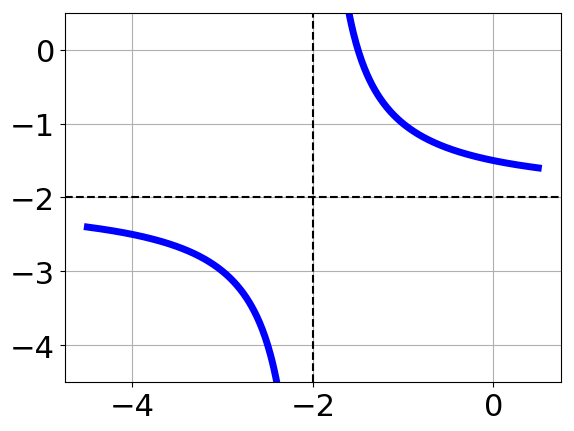
\includegraphics[width=0.3\textwidth]{../Figures/rationalEquationToGraphBB.png} \end{center}\begin{tabular}{|c|c|} 
\hline 
 & \tabularnewline 
 \textbf{A.} 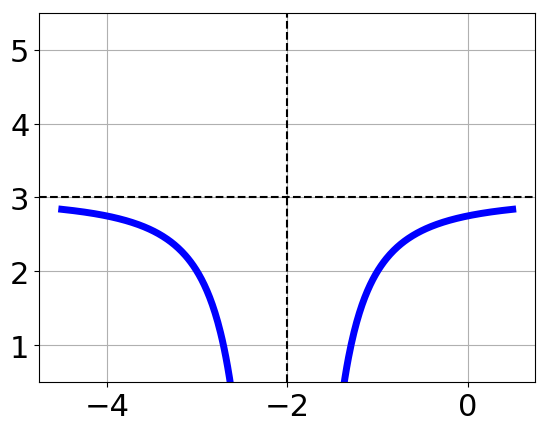
\includegraphics[width=0.3\textwidth]{../Figures/rationalEquationToGraphAB.png} & \textbf{B.} 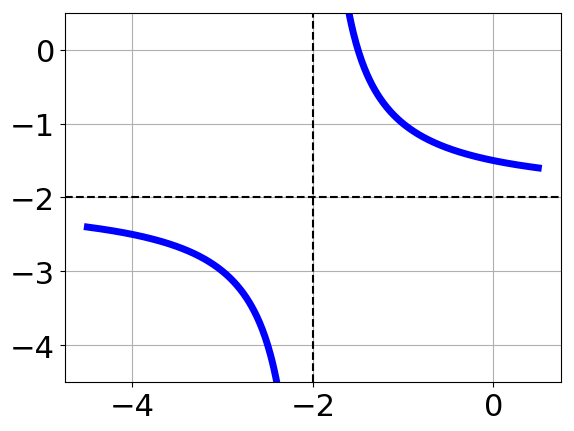
\includegraphics[width=0.3\textwidth]{../Figures/rationalEquationToGraphBB.png} \tabularnewline 
\hline 
 & \tabularnewline 
 \textbf{C.} 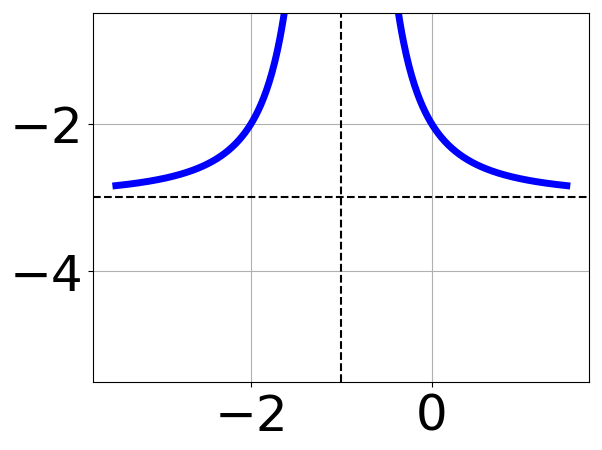
\includegraphics[width=0.3\textwidth]{../Figures/rationalEquationToGraphCB.png} & \textbf{D.} 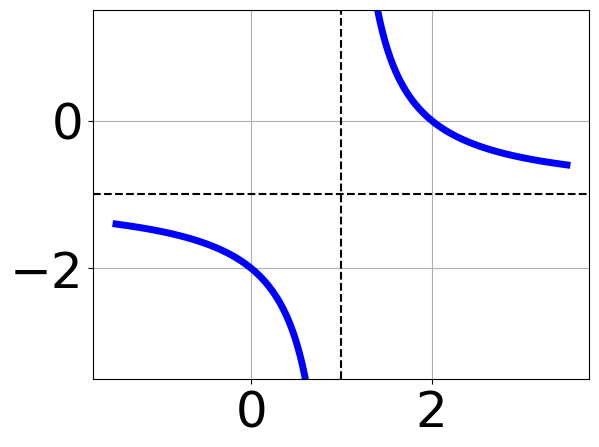
\includegraphics[width=0.3\textwidth]{../Figures/rationalEquationToGraphDB.png} \tabularnewline 
\hline 
 E. None of the figures above. & \tabularnewline 
\hline 
 \end{tabular} 
 
\begin{enumerate}[label=\Alph*.] 
\item This is the correct option.  
\item Corresponds to using the general form $f(x) = \frac{a}{(x+h)^2}+k$ and the opposite leading coefficient.  
\item Corresponds to thinking the graph was a shifted version of $\frac{1}{x}$.  
\item Corresponds to thinking the graph was a shifted version of $\frac{1}{x}$, using the general form $f(x) = \frac{a}{(x+h)^2}+k$, and the opposite leading coefficient.  
\end{enumerate} 
 
\textbf{General Comment:} General Comments: Remember that the general form of a basic rational equation is $ f(x) = \frac{a}{(x-h)^n} + k$, where $a$ is the leading coefficient (and in this case, we assume is either $1$ or $-1$), $n$ is the degree (in this case, either $1$ or $2$), and $(h, k)$ is the intersection of the asymptotes. 

-----------------------------------------------

3. Solve the rational equation below. Then, choose the interval(s) that the solution(s) belongs to.
\[ \frac{-7x}{-5x -2} + \frac{-3x^{2}}{10x^{2} +24 x + 8} = \frac{-4}{-2x -4} \] 
The solution is $ \text{There are two solutions: } x = 0.563 \text{ and } x = -1.291 $ 

\begin{enumerate}[label=\Alph*.] 
\item $ x \in [-1.93,-0.91] $ 

  
\item $ \text{All solutions lead to invalid or complex values in the equation.} $ 

  
\item $ x_1 \in [0.1, 3.44] \text{ and } x_2 \in [-1.66,-1.12] $ 

 * $x = 0.563 \text{ and } x = -1.291$, which is the correct option. 
\item $ x_1 \in [0.1, 3.44] \text{ and } x_2 \in [-0.46,-0.07] $ 

  
\item $ x \in [-2.7,-1.86] $ 

  
\end{enumerate} 
 
\textbf{General Comment:} General Comments: Distractors are different based on the number of solutions. Remember that after solving, we need to make sure our solution does not make the original equation divide by zero! 

-----------------------------------------------

4. Determine the domain of the function below.
\[ f(x) = \frac{4}{30x^{2} +54 x + 24} \] 
The solution is $ \text{All Real numbers except } x = -1.000 \text{ and } x = -0.800. $ 

\begin{enumerate}[label=\Alph*.] 
\item $ \text{All Real numbers except } x = a \text{ and } x = b, \text{ where } a \in [-36.56, -35.81] \text{ and } b \in [-20.38, -19.72] $ 

 All Real numbers except $x = -36.000$ and $x = -20.000$, which corresponds to not factoring the denominator correctly. 
\item $ \text{All Real numbers except } x = a \text{ and } x = b, \text{ where } a \in [-1.21, -0.9] \text{ and } b \in [-0.89, -0.45] $ 

 All Real numbers except $x = -1.000$ and $x = -0.800$, which is the correct option. 
\item $ \text{All Real numbers except } x = a, \text{ where } a \in [-1.21, -0.9] $ 

 All Real numbers except $x = -1.000$, which corresponds to removing only 1 value from the denominator. 
\item $ \text{All Real numbers except } x = a, \text{ where } a \in [-36.56, -35.81] $ 

 All Real numbers except $x = -36.000$, which corresponds to removing a distractor value from the denominator. 
\item $ \text{All Real numbers.} $ 

 This corresponds to thinking the denominator has complex roots or that rational functions have a domain of all Real numbers. 
\end{enumerate} 
 
\textbf{General Comment:} General Comments: The new domain is the intersection of the previous domains. 

-----------------------------------------------

0. Solve the rational equation below. Then, choose the interval(s) that the solution(s) belongs to.
\[ \frac{9}{-2x + 6} + 5 = \frac{6}{18x -54} \] 
The solution is $ x = 3.967 $ 

\begin{enumerate}[label=\Alph*.] 
\item $ x \in [3.97,4.97] $ 

 * $x = 3.967$, which is the correct option. 
\item $ \text{All solutions lead to invalid or complex values in the equation.} $ 

 This corresponds to thinking $x = 3.967$ leads to dividing by zero in the original equation, which it does not. 
\item $ x_1 \in [-3, -1.7] \text{ and } x_2 \in [2,6] $ 

 $x = -2.033 \text{ and } x = 3.967$, which corresponds to getting the correct solution and believing there should be a second solution to the equation. 
\item $ x \in [-3,-1.7] $ 

 $x = -2.033$, which corresponds to not distributing the factor $-2x + 6$ correctly when trying to eliminate the fraction. 
\item $ x_1 \in [3.1, 3.7] \text{ and } x_2 \in [2,6] $ 

 $x = 3.300 \text{ and } x = 3.967$, which corresponds to getting the correct solution and believing there should be a second solution to the equation. 
\end{enumerate} 
 
\textbf{General Comment:} General Comments: Distractors are different based on the number of solutions. Remember that after solving, we need to make sure our solution does not make the original equation divide by zero! 

-----------------------------------------------


\end{document}

